\section{Video Transcoder}
\label{sec:video_transcoder}

Once the upload process described is ended, the transcoding phase begins. The video uploaded on S3 is taken over and processed by Elastic Transcoder, and will produce a file with a .m3u8 format in output. This allows the HLS streaming with the advantages illustrated in the previous chapters. The follwing image shows the general function and idea of where the stream that starts from Bucket S3 goes through a TranscodingPipeline where the video is converted and uploaded to S3 once again.


\begin{figure}[htb]
 \centering
 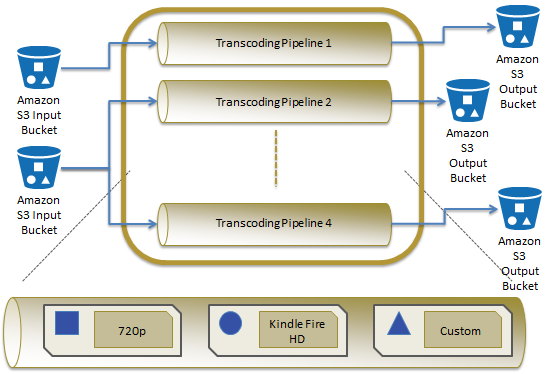
\includegraphics[width=1.0\linewidth]{images/chapter6/elastic_transcode_model.png}\hfill
 \caption[The Elastic Transcoder Model]{The Elastic Transcoder Model}
 \label{fig:fourV}
\end{figure}
In detail, the transcoding begins at the end of the MultipartUpload when the server calls API PUT /transcoders/createJob which takes in input the following parameters:

\begin{itemize}
      \item file\_name is the file name that must be taken from the bucket so it can later be transformed.

      \item path is the remote path where the storage can be put into effect when the transcoding is completed.
  \end{itemize}
This API begins the comunication with the ElasticTranscoder service and in this way creates a new JOB which will be inserted into the Pipeline that is specified in the PipelineID field.

\begin{lstlisting}[language=html]
  
Transcoder.createJob = function (file_name,path,callback){
    var input_params = {
      Input: { 
        Key: file_name, 
        FrameRate: 'auto', 
        Resolution: 'auto', 
        AspectRatio: 'auto', 
        Interlaced: 'auto', 
        Container: 'auto' 
      }, 
      PipelineId: PIPELINE_ID, // specifies output/input buckets in S3 
      OutputKeyPrefix: path,
      Output: { 
        Key: file_name, 
        PresetId: PRESET_ID, // specifies the output video format
        SegmentDuration: '5',
        ThumbnailPattern:'image/' + file_name + '-{count}'//modifica preset per determinare il numero di immagini
      },

    };    
    elastictranscoder.createJob(input_params, function(err, data) {
      if (err) {
        console.log(err, err.stack); // an error occurred
        callback(err);
        return;
      }else{
        callback(null, data);
      }
    });
  };
  
  Transcoder.remoteMethod('createJob', {
    http: { verb: 'put' },
    accepts: [
      {arg: 'file_name', type: 'string'},
      {arg: 'path', type: 'string'}
    ],
    returns: {arg: 'dataId', type: 'string'}
  });
\end{lstlisting}

In the following code, it can be seen how the server in the request specifies a PipelineID. This is an ID that corrisponds to a certain Pipeline, where the job in question will be inserted.

Another parameter necessary requested by the API is the PresetID, which represents the ID of the Preset. The Preset see(\ref{sec:Amazon Elastic Transcoder}) is a template that contains most of the settings for transcoding media files from one format to another.

The following image shows the Pipeline used during the testing phase of the X-learning platform.

\begin{minipage}{\linewidth}
    \centering
    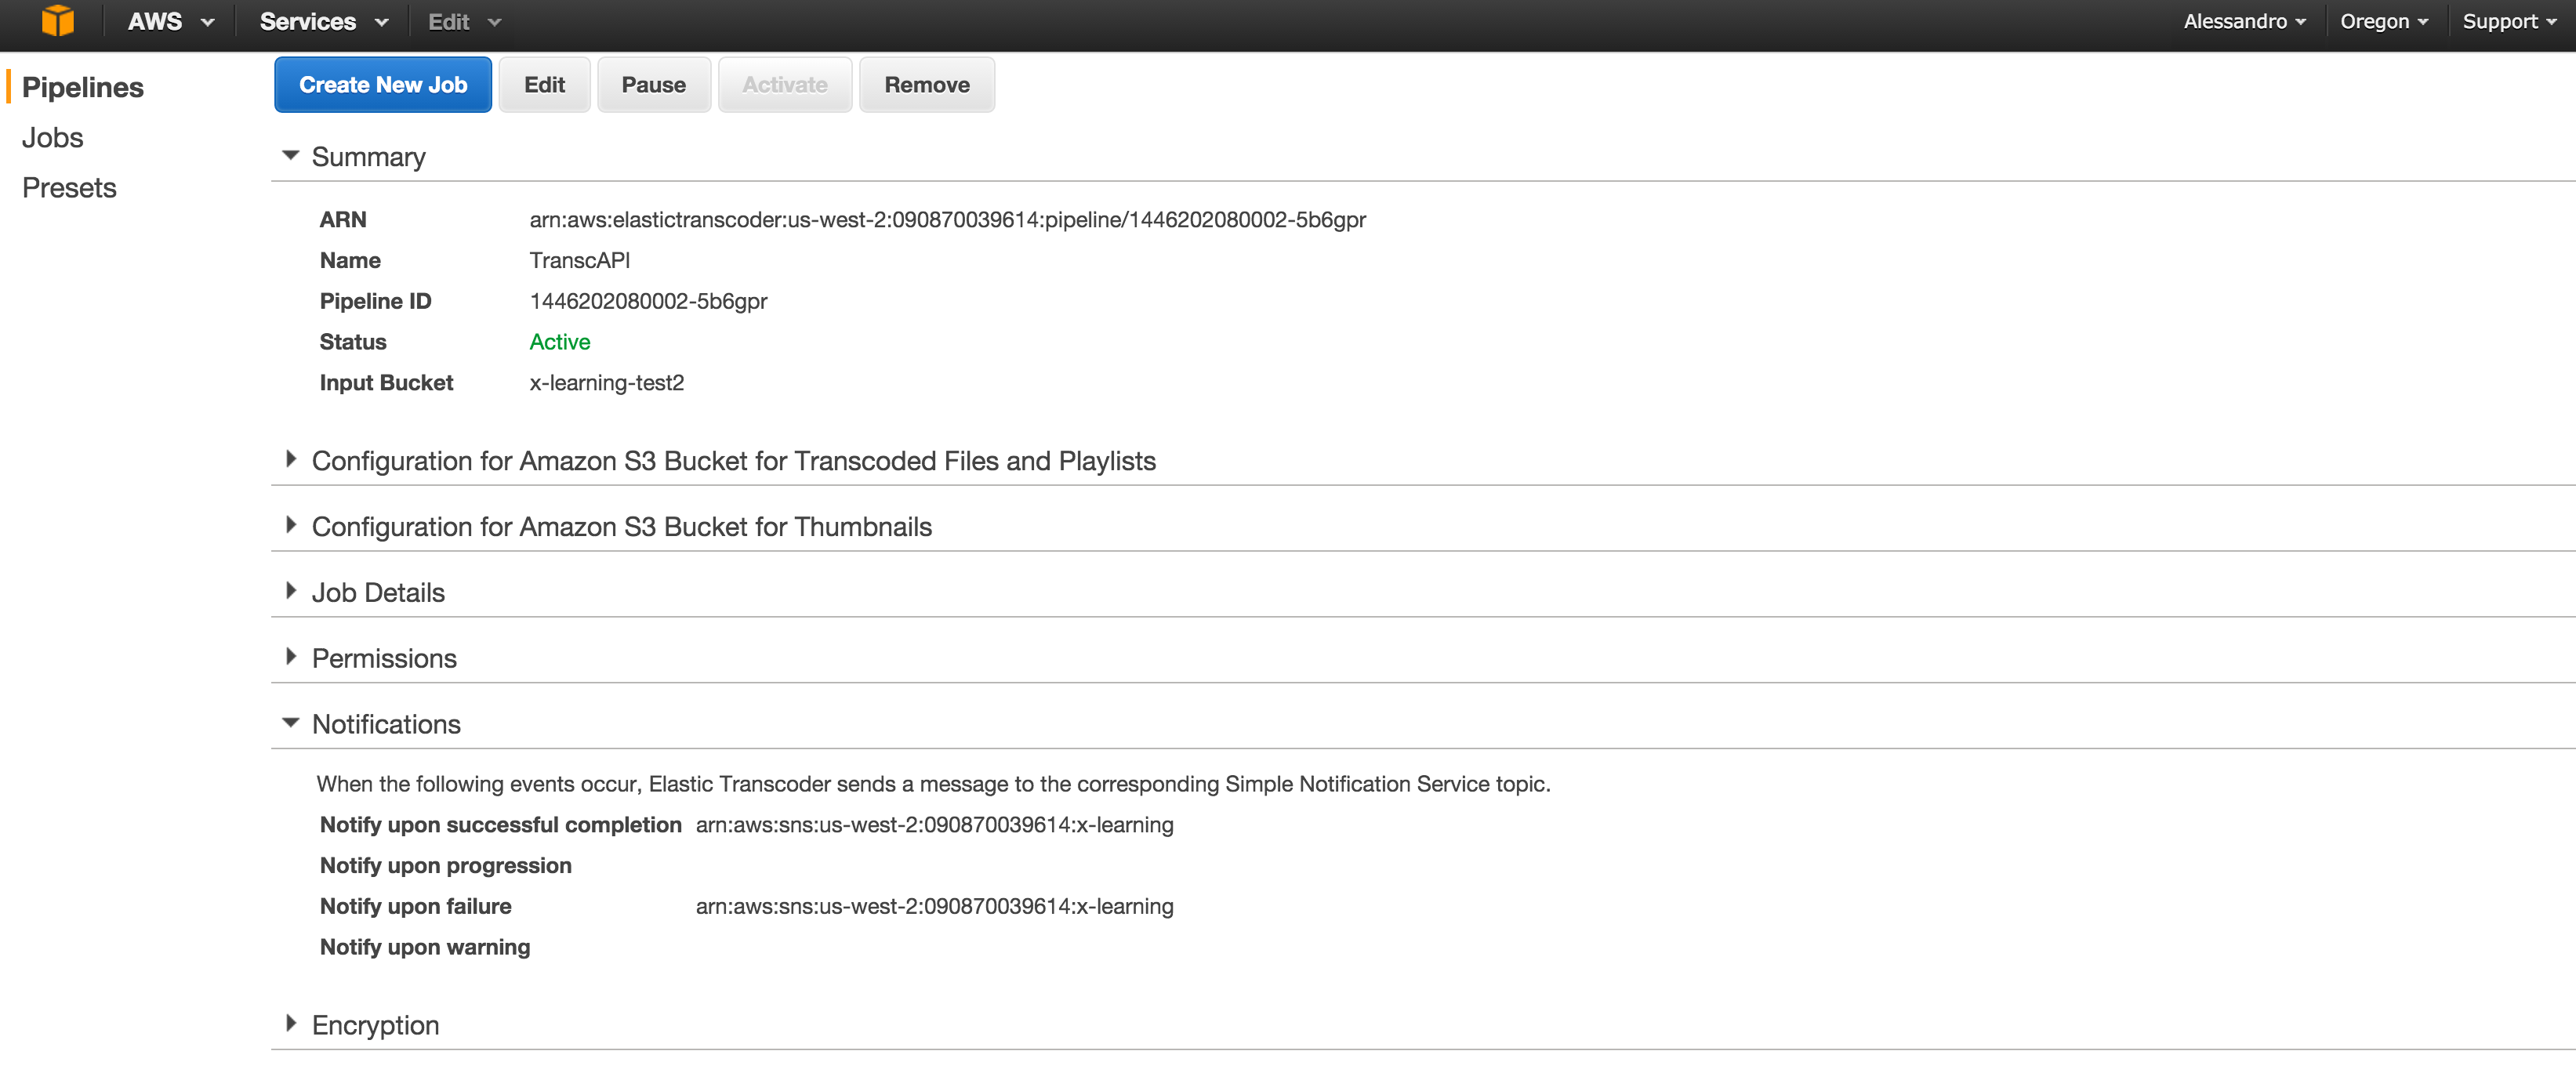
\includegraphics[width=1.0\linewidth]{images/chapter6/elastic_pipeline.png}
    \captionof{figure}[Web Components]{X-Learning Pipeline}
\end{minipage}
It is also possible to see how in the Pipeline “arn:aws:sns:us-west-2:090870039614:x-learning” is specified, which represents the Amazon Simple Notification Service that is a distributed publish-subscribe system. 
This service see(\ref{sec:Amazon SNS and SQS}) is used with the SQS service, which is a queue with the transcoding results.

These results within the SQS are received as notifications by the platform that the server side analyzes in order to:


\begin{itemize}
\item make the course available for publication and accessible to students (Member).

\item free up space on the S3 bucket by eliminating the video in the original format.

\begin{lstlisting}[language=javascript]

sqs.receiveMessage(receiveMessageParams, receiveMessageCallback);

  function receiveMessageCallback(err, data) {
    if (data.Messages && data.Messages.length > 0) {
      var message = JSON.parse(data.Messages[0].Body);
      var key = JSON.parse(message.Message).input.key;
      
      // Delete the message when we've successfully processed it
      var deleteMessageParams = {
        QueueUrl: queueUrl,
        ReceiptHandle: data.Messages[0].ReceiptHandle
      };

      var s3_params = {
        Bucket: S3_BUCKET,
        Delete: { 
          Objects: [ 
            {
              Key: key
            }
          ]
        }
      };
      s3.deleteObjects(s3_params,deleteObjCallback)
      sqs.deleteMessage(deleteMessageParams, deleteMessageCallback);
    }
    \end{lstlisting}

\end{itemize}




